\documentclass[aspectratio=169,10pt]{beamer}
\usetheme[compress,subsection=false]{Berlin}
\usepackage[T1]{fontenc}
\usepackage{lmodern}
\usepackage{booktabs,tabularx,array}
\usepackage{tikz,pgfplots}
\usetikzlibrary{arrows.meta,positioning,calc}
\usepgfplotslibrary{groupplots}
\pgfplotsset{compat=1.18}
\definecolor{navy}{HTML}{004B7A}
\definecolor{ink}{HTML}{173449}
\definecolor{muted}{HTML}{5C6F7D}
\definecolor{forecast}{HTML}{267FB4}
\definecolor{current}{HTML}{16877F}
\definecolor{longfade}{HTML}{BD732B}
\definecolor{survival}{HTML}{7A5F9E}
\definecolor{alertred}{HTML}{BE5348}
\definecolor{pale}{HTML}{F0F5F8}
\setbeamercolor{normal text}{fg=ink,bg=white}
\setbeamercolor{structure}{fg=navy}
\setbeamercolor{alerted text}{fg=alertred}
\setbeamercolor{block title}{fg=navy,bg=pale}
\setbeamercolor{block body}{fg=ink,bg=pale}
\setbeamerfont{frametitle}{size=\Large,series=\bfseries}
\setbeamerfont{block title}{size=\normalsize}
\setbeamercolor{frametitle}{fg=white,bg=navy}
\setbeamertemplate{navigation symbols}{}
\setbeamertemplate{itemize item}{\small\raisebox{.15ex}{\textbullet}}
\setbeamersize{text margin left=8mm,text margin right=8mm}
\setbeamertemplate{footline}{\leavevmode\hbox to\paperwidth{\hskip8mm%
  \textcolor{muted}{\scriptsize Giuseppe Gabriele Russo\quad |\quad Satellite Link Fade Nowcasting}%
  \hfil\textcolor{muted}{\scriptsize\insertframenumber\,/\,\inserttotalframenumber}\hskip3mm%
  \raisebox{-1mm}{
\includegraphics[height=6mm]{../figures/cherubino_pant541.png}}\hskip8mm}\vskip3mm}
\newcommand{\takeaway}[1]{\vfill\begin{beamercolorbox}[sep=2mm,wd=\textwidth]{block body}\small\textbf{#1}\end{beamercolorbox}}
\newcommand{\smallnote}[1]{\par\vspace{2mm}{\scriptsize\color{muted}#1\par}}
\newcommand{\rulebox}[1]{\begin{block}{Decision before shared post-processing}\centering #1\end{block}}
\pgfplotsset{every axis/.append style={
  font=\footnotesize,axis line style={muted!50},tick style={muted!40},
  grid=major,grid style={muted!12},
  label style={font=\footnotesize},tick label style={font=\scriptsize},
  legend style={font=\scriptsize,draw=none,fill=none},
  scaled ticks=false}}
\title{Machine Learning for Satellite Link Fade Nowcasting}
\author{Giuseppe Gabriele Russo}
\date{}
\hypersetup{pdftitle={Machine Learning for Satellite Link Fade Nowcasting},pdfauthor={Giuseppe Gabriele Russo}}

\begin{document}

\section{Introduction}

% 1 -- 0:20
\begin{frame}[plain]
  \begin{minipage}{.68\textwidth}
    
\includegraphics[height=17mm]{../figures/cherubino_pant541.png}\hspace{4mm}%
    \begin{minipage}{.72\linewidth}\color{navy}\textbf{University of Pisa}\\[1mm]
    \small Master's Degree in Computer Science\\Curriculum: Artificial Intelligence\end{minipage}
  \end{minipage}\hfill
\includegraphics[width=27mm]{mbi.png}
  \vspace{10mm}

  {\color{navy}\LARGE\bfseries Machine Learning for\\[2mm] Satellite Link Fade Nowcasting\par}
  \vspace{5mm}
  {\large Giuseppe Gabriele Russo\par}
  \vspace{2mm}
  {\color{muted}Experimental thesis carried out at M.B.I. S.r.l.\par}
  \vfill
  \begin{columns}[T,onlytextwidth]
    \column{.48\textwidth}\small\textcolor{muted}{Supervisor}\\\textbf{Davide Bacciu}
    \column{.48\textwidth}\small\textcolor{muted}{Co-supervisor}\\\textbf{Giovanni Scognamiglio}
  \end{columns}
  \vspace{4mm}
\end{frame}

% 2 -- 1:20
\begin{frame}{Industrial Context and Operational Problem}
\begin{columns}[T,onlytextwidth]
\column{.40\textwidth}
\textbf{Experimental work at M.B.I.}\\[2mm]
Real satellite fade and beacon recordings from the Fucino ground station.
\vspace{4mm}
\begin{block}{The operational question}
Will the fade persist long enough to justify a backup-link switch?
\end{block}
\column{.57\textwidth}
\begin{tikzpicture}
\begin{axis}[width=\linewidth,height=4.4cm,xmin=0,xmax=60,ymin=0,ymax=45,
 xlabel={Time from window start (min)},ylabel={Signal (dB)},legend pos=north east]
\addplot[ink,thick] table[x=minutes,y=signal,col sep=comma]{data/event.csv};
\addlegendentry{Observed signal}
\addplot[alertred,dashed,thick] coordinates {(0,10)(60,10)};
\addlegendentry{10 dB threshold}
\end{axis}
\end{tikzpicture}
\smallnote{Except from the held-out source; future samples are unavailable to the predictor at decision time.}
\end{columns}
\takeaway{Anticipate persistence, rather than only detect a threshold crossing.}
\end{frame}

% 3 -- 1:00
\begin{frame}{Research Objective and Contribution}
\leavevmode{\large Which predictive formulation supports useful switch decisions\\from signal history alone?\par}
\vspace{1mm}
{\centering
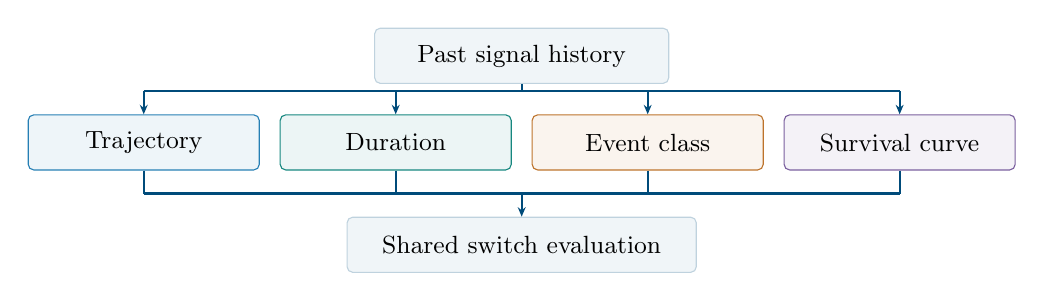
\begin{tikzpicture}[box/.style={draw=navy!25,fill=pale,rounded corners=2pt,align=center,minimum height=7mm,font=\small},>={Stealth[length=1.2mm,width=1mm]}]
\node[box,text width=35mm] (history) at (0,1) {Past signal history};
\node[box,text width=27mm,draw=forecast,fill=forecast!8] (trajectory) at (-4.8,-0.1) {Trajectory};
\node[box,text width=27mm,draw=current,fill=current!8] (duration) at (-1.6,-0.1) {Duration};
\node[box,text width=27mm,draw=longfade,fill=longfade!8] (event) at (1.6,-0.1) {Event class};
\node[box,text width=27mm,draw=survival,fill=survival!8] (curve) at (4.8,-0.1) {Survival curve};
\node[box,text width=42mm] (decision) at (0,-1.4) {Shared switch evaluation};
\draw[thick,navy] (history.south)--(0,.55);
\draw[thick,navy] (-4.8,.55)--(4.8,.55);
\draw[thick,navy] (-4.8,-.75)--(4.8,-.75);
\foreach \target in {trajectory,duration,event,curve}{
  \draw[->,thick,navy] (\target.north |- 0,.55)--(\target.north);
  \draw[thick,navy] (\target.south)--(\target.south |- 0,-.75);
}
\draw[->,thick,navy] (0,-.75)--(decision.north);
\end{tikzpicture}
\par}
\vspace{3mm}
\begin{itemize}\setlength{\itemsep}{1.5mm}
\item Compare four task formulations using established model families.
\item Separate predictive accuracy from operational switch behavior.
\item Make decision coverage explicit when comparing different tasks.
\end{itemize}
\end{frame}

% 4 -- 1:10
\begin{frame}{Data and Experimental Setting}
\noindent
{\small\color{muted}Signal-only inputs \quad 30-second sampling \quad Main context: 30 observations\par}
\vspace{3mm}
\begin{columns}[T,onlytextwidth]
\column{.51\textwidth}
\textbf{Why sample around fades?}\par\vspace{2mm}
Fade episodes are sparse; most samples lie near the non-fade baseline.
\par\vspace{2mm}
\small Uniform sampling risks letting long quiet plateaus dominate the training loss.
\par\vspace{3mm}
\textcolor{navy}{\textbf{Event-focused sample selection}}\par\vspace{1mm}
Forecasting / current-level: windows extending \textbf{90 min before and after} candidate onset.\\[2mm]
Long-fade / survival: \textbf{within-event samples}.
\column{.43\textwidth}
\begin{block}{Development sources}
Chronological training / validation splits.\\[2mm]
Validation-based model selection.
\end{block}
\vspace{2mm}
\begin{block}{External test source}
\texttt{fc-uplink-fade.csv}\\[2mm]
Excluded from fitting and hyperparameter search.
\end{block}
\end{columns}
\takeaway{Event-focused evaluation is not continuous monitoring of the complete time series.}
\end{frame}

% 5 -- 1:20
\section{Methodology}
\begin{frame}{Four Predictive Formulations}
\renewcommand{\arraystretch}{1.7}
\begin{tabularx}{\textwidth}{@{}p{36mm}X p{39mm}@{}}
\toprule
\textbf{Formulation} & \textbf{Question at time $t$} & \textbf{Output}\\\midrule
\textcolor{forecast}{\textbf{Autoregressive}} & What are the next ten signal values? & Future trajectory\\
\textcolor{current}{\textbf{Current-level}} & How long until the signal falls below the threshold $S_t-0.5$ dB? & Duration estimate\\
\textcolor{longfade}{\textbf{Long-fade}} & Does the entire grouped event last at least 300 seconds? & Class probability\\
\textcolor{survival}{\textbf{Survival}} & Will the current fade remain active for more than $u$ seconds? & Survival curve $S(u\mid X_t)$\\
\bottomrule
\end{tabularx}
\takeaway{All use past signal information; their targets are not interchangeable.}
\end{frame}

% 6 -- 0:55
\begin{frame}{Perfect Switch and Evaluation}
\begin{columns}[T,onlytextwidth]
\column{.46\textwidth}
\begin{block}{Perfect Switch}
An offline reference using the true signal and future persistence.\\[2mm]
An evaluation oracle, not a deployable predictor.
\end{block}
\vspace{2mm}
\textbf{Complementary measurements}
\begin{itemize}
\item Precision, recall, F1, balanced accuracy.
\item Active duration and switch intervals.
\item Timing and missed activity.
\end{itemize}
\column{.49\textwidth}
\vspace{8mm} % sposta il grafico più in basso
\hspace{9mm} % sposta il grafico più a destra
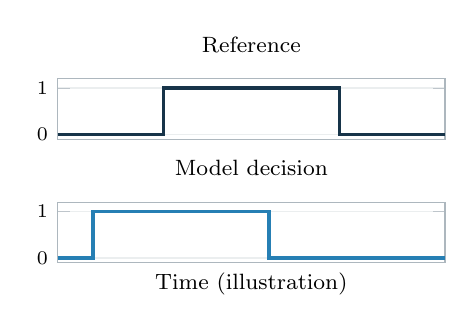
\begin{tikzpicture}
\begin{groupplot}[group style={group size=1 by 2,vertical sep=8mm},width=6.5cm,height=2.35cm,
 xmin=0,xmax=11,ymin=-.1,ymax=1.2,ytick={0,1},xtick=\empty]
\nextgroupplot[title={Reference}]
\addplot[const plot,ink,very thick] coordinates {(0,0)(3,1)(8,0)(11,0)};
\nextgroupplot[title={Model decision},xlabel={Time (illustration)}]
\addplot[const plot,forecast,very thick] coordinates {(0,0)(1,1)(6,0)(11,0)};
\end{groupplot}
\end{tikzpicture}
\end{columns}
\vspace{2mm}
\takeaway{Measure what the decision does, not only how accurate the prediction is.}
\end{frame}

% 7 -- 1:05
\begin{frame}{Shared Switch Post-Processing}
\begin{columns}[T,onlytextwidth]
\column{.39\textwidth}
\vspace{2mm}
\textbf{1. Raw decision}\\
Apply the task-specific conversion rule.
\vspace{4mm}

\textbf{2. Minimum active interval}\\
Extend short positive islands to the configured ten-sample length.
\vspace{4mm}

\textbf{3. Hold while above threshold}\\
Keep an already active switch on while the current signal remains $\geq10$ dB.
\smallnote{Modifies the binary decision, not the input signal.}
\column{.58\textwidth}
\begin{tikzpicture}
\begin{groupplot}[group style={group size=1 by 4,vertical sep=2mm},width=7cm,height=1.12cm,
 scale only axis,xmin=1,xmax=15,xtick=\empty,ymin=-.15,ymax=1.2,ytick={0,1},ylabel style={font=\scriptsize}]
\nextgroupplot[ymin=8.5,ymax=11.5,ytick={9,11},ylabel={Signal}]
\addplot[ink,thick] table[x=sample,y=signal,col sep=comma]{data/postprocessing.csv};
\addplot[alertred,dashed] coordinates{(1,10)(15,10)};
\nextgroupplot[ylabel={Raw}]
\addplot[const plot,forecast,thick] table[x=sample,y=raw,col sep=comma]{data/postprocessing.csv};
\nextgroupplot[ylabel={Extended}]
\addplot[const plot,survival,thick] table[x=sample,y=extended,col sep=comma]{data/postprocessing.csv};
\nextgroupplot[ylabel={Final},xtick={1,5,10,15},xlabel={Sample (30 seconds)}]
\addplot[const plot,current,very thick] table[x=sample,y=held,col sep=comma]{data/postprocessing.csv};
\end{groupplot}
\end{tikzpicture}
\end{columns}
\end{frame}

% 8 -- 1:40
\section{Models}
\begin{frame}{Autoregressive Forecasting}
\noindent
{\small\color{muted}GRU S2V / encoder--decoder \quad PatchTST \quad XGBoost \quad Chronos\par}
\vspace{4mm}
\begin{columns}[T,onlytextwidth]
\column{.44\textwidth}
\textcolor{forecast}{\textbf{Predict}}\par\vspace{2mm}
\textbf{30 past values} $\longrightarrow$ \textbf{10 future values}.
\vspace{3mm}

\small Trainable models: raw and context-standardized inputs. Chronos: raw, zero-shot.
\vspace{3mm}
\begin{block}{Initial switch}
All ten predictions are $\geq10$ dB.
\end{block}
\column{.50\textwidth}
\textbf{Forecast error vs. switch quality}\par
\vspace{3mm}
\renewcommand{\arraystretch}{1.8}
\begin{tabular}{@{}lrr@{}}\toprule
Model & RMSE (dB) $\downarrow$ & Switch F1 $\uparrow$\\\midrule
GRU S2V raw & \textbf{2.852} & 0.674\\
PatchTST raw & 3.088 & \textbf{0.808}\\\bottomrule
\end{tabular}\par
\smallnote{External test, native L30 grid.}
\end{columns}
\takeaway{Lower forecast error does not guarantee better switches.}
\end{frame}

% 9 -- 1:25
\begin{frame}{Current-Level Persistence}
\noindent
{\small\color{muted}XGBoost \quad Shapelets with MLP, convolutional or Transformer heads\par}
\vspace{4mm}
\begin{columns}[T,onlytextwidth]
\column{.44\textwidth}
\textcolor{current}{\textbf{Predict}}\par\vspace{2mm}
Time until the signal falls below its \textbf{current level minus 0.5 dB}.
\par\vspace{3mm}
\small Input: relative-to-current history plus scalar signal features.
\vspace{3mm}
\begin{block}{Initial switch}
Predicted duration $\geq5$ min\\
and current signal $\geq10$ dB.
\end{block}
\column{.50\textwidth}
\hspace{6mm}
\textbf{XGBoost: duration vs. decision}\par
\vspace{3mm}
\renewcommand{\arraystretch}{1.5}
\hspace{6mm}
\begin{tabular}{@{}lr@{}}\toprule
Duration MAE $\downarrow$ & \textbf{586.9 s}\\
Duration median AE $\downarrow$ & 27.2 s\\\midrule
Switch F1 $\uparrow$ & \textbf{0.902}\\\bottomrule
\end{tabular}\par
\hspace{6mm}
\smallnote{External test, native grid.}
\vspace{2mm}
\small\textbf{Shapelet variants:} no final switch activations on this test set.
\end{columns}
\takeaway{Useful switches despite large errors; level recovery is not fade recovery.}
\end{frame}

% 10 -- 1:20
\begin{frame}{Long-Fade Detection}
\noindent
{\small\color{muted}XGBoost \quad TCN \quad Shapelet convolution classifier\par}
\vspace{4mm}
\begin{columns}[T,onlytextwidth]
\column{.44\textwidth}
\textcolor{longfade}{\textbf{Predict}}\par\vspace{2mm}
Probability that the \textbf{whole grouped event} lasts at least 5 min.
\par\vspace{3mm}
\small The label stays the same throughout the event, even near its end.
\vspace{3mm}
\begin{block}{Initial switch}
Predicted probability $\geq0.5$.
\end{block}
\column{.50\textwidth}
\hspace{6mm}
\textbf{TCN: classification vs. decision}\par
\vspace{3mm}
\renewcommand{\arraystretch}{1.6}
\hspace{6mm}
\begin{tabular}{@{}lr@{}}\toprule
Classification AUPRC $\uparrow$ & $\approx1.000$\\\midrule
Switch precision $\uparrow$ & \textbf{0.540}\\
Switch recall $\uparrow$ & \textbf{1.000}\\\bottomrule
\end{tabular}\par
\smallnote{External test, native grid. Event-conditioned, highly imbalanced classification.}
\end{columns}
\takeaway{Total event duration is not remaining duration.}
\end{frame}

% 11 -- 1:35
\begin{frame}{Survival Persistence}
\noindent
{\small\color{muted}XGBoost-AFT: time distribution \qquad TCN: discrete hazards\par}
\vspace{2mm}
\begin{columns}[T,onlytextwidth]
\column{.42\textwidth}
\textcolor{survival}{\textbf{Remaining fade duration}}
\[
\mathcal S(u\mid X_t)=P(R_t>u\mid X_t)
\]
\small Right-censored samples are retained.
\vspace{2mm}
\begin{block}{Initial switch}
Five-minute probability $\geq0.65$\\
and current signal $\geq10$ dB.
\end{block}
\smallnote{\textcolor{alertred}{0.65 is exploratory/test-selected, not validation-calibrated.}}
\column{.54\textwidth}
\begin{tikzpicture}
\begin{axis}[width=\linewidth,height=4.1cm,xmin=0,xmax=30,ymin=0,ymax=1,
 xlabel={Remaining time (min)},ylabel={Survival probability},legend pos=north east]
\addplot[forecast,very thick] table[x=minutes,y=curve1,col sep=comma]{data/survival.csv};\addlegendentry{Low $S(300)$}
\addplot[current,very thick] table[x=minutes,y=curve2,col sep=comma]{data/survival.csv};\addlegendentry{Median $S(300)$}
\addplot[survival,very thick] table[x=minutes,y=curve3,col sep=comma]{data/survival.csv};\addlegendentry{High $S(300)$}
\addplot[muted,dashed] coordinates{(5,0)(5,1)};
\end{axis}
\end{tikzpicture}
\smallnote{Three test TCN predictions; dashed line: 5 min.}
\end{columns}
\vspace{2mm}
\takeaway{Direct residual-persistence estimates, with calibration still required.}
\end{frame}

% 12 -- 1:20
\section{Results}
\begin{frame}{Cross-Task Switch Performance}
\textbf{Selected representatives on the common reference grid}\par
\vspace{3mm}
\renewcommand{\arraystretch}{1.4}
\setlength{\tabcolsep}{4pt}
\noindent\begin{tabularx}{\textwidth}{@{}Xrrrr@{}}\toprule
Representative & Coverage & Precision $\uparrow$ & Recall $\uparrow$ & F1 $\uparrow$\\\midrule
\textcolor{current}{Current-level XGBoost} & 89.0\% & \textbf{1.000} & 0.808 & \textbf{0.894}\\
\textcolor{survival}{Survival XGBoost-AFT} & 9.2\% & 0.812 & 0.938 & 0.870\\
\textcolor{forecast}{PatchTST raw} & 89.2\% & 0.779 & 0.821 & 0.800\\
\textcolor{longfade}{Long-fade TCN} & 28.7\% & 0.557 & \textbf{1.000} & 0.715\\\bottomrule
\end{tabularx}\par
\vspace{3mm}
\small Missing native decisions map to zero. Coverage measures the fraction of reference timestamps with a native decision.
\smallnote{Survival threshold: exploratory 0.65. Descriptive test comparison, not a validation-selected cross-task winner.}
\takeaway{Conservative activation, greater recovery and broad recall are different trade-offs.}
\end{frame}

% 13 -- 1:40
\begin{frame}{Active Duration and Switching Events}
\begin{columns}[T,onlytextwidth]
\column{.61\textwidth}
\vspace{10mm} % sposta il grafico più in basso
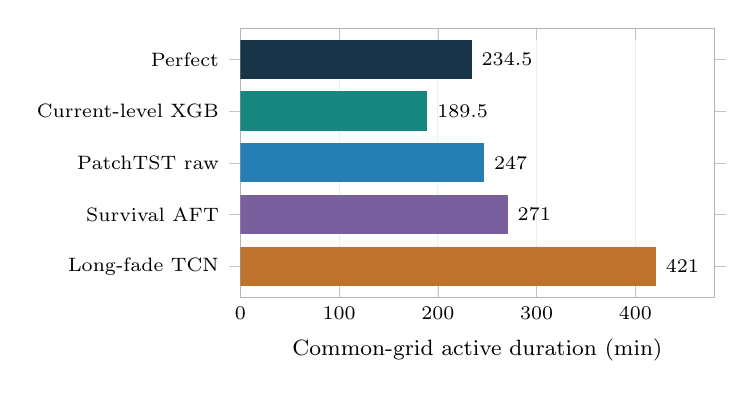
\begin{tikzpicture}
\begin{axis}[xbar,bar shift=0,width=7.6cm,height=5cm,xmin=0,xmax=480,ymin=-.6,ymax=4.6,
 ytick={0,1,2,3,4},yticklabels={Long-fade TCN,Survival AFT,PatchTST raw,Current-level XGB,Perfect},
 xlabel={Common-grid active duration (min)},bar width=5mm,
 nodes near coords,nodes near coords style={font=\scriptsize},
 yticklabel style={font=\scriptsize},xmajorgrids=true,ymajorgrids=false]
\addplot[fill=ink,draw=none] coordinates{(234.5,4)};
\addplot[fill=current,draw=none] coordinates{(189.5,3)};
\addplot[fill=forecast,draw=none] coordinates{(247,2)};
\addplot[fill=survival,draw=none] coordinates{(271,1)};
\addplot[fill=longfade,draw=none] coordinates{(421,0)};
\end{axis}
\end{tikzpicture}
\column{.35\textwidth}
\textbf{Duration is not fragmentation}
\vspace{3mm}

The same active time can be split into very different numbers of switch intervals.
\vspace{4mm}
\begin{block}{Within-task example}
Native autoregressive grid:\\[2mm]
Perfect: \textbf{18 intervals}\\
PatchTST: \textbf{20 intervals}
\end{block}
\smallnote{An interval is a contiguous run of switch 1, not necessarily a distinct physical fade. Native counts are not cross-task counts.}
\end{columns}
\end{frame}

% 14 -- 1:20
\begin{frame}{An Event-Level Comparison}
\vspace{-3mm}
\begin{center}
\begin{tikzpicture}
\begin{groupplot}[group style={group size=1 by 6,vertical sep=2mm},width=11.6cm,height=.51cm,
 scale only axis,xmin=0,xmax=180,xtick={0,30,60,90,120,150,180},xticklabels=\empty,
 ymin=-.15,ymax=1.2,ytick=\empty,ymajorgrids=false]
\nextgroupplot[height=1.1cm,ymin=0,ymax=40,ytick={0,20,40},ylabel={Signal (dB)}]
\addplot[ink,thick] table[x=minutes,y=signal,col sep=comma]{data/event.csv};
\addplot[alertred,dashed] coordinates{(0,10)(180,10)};
\nextgroupplot
\addplot[const plot,ink,very thick] table[x=minutes,y=perfect,col sep=comma]{data/event.csv};
\nextgroupplot
\addplot[const plot,current,very thick] table[x=minutes,y=current,col sep=comma]{data/event.csv};
\nextgroupplot
\addplot[const plot,forecast,very thick] table[x=minutes,y=forecast,col sep=comma]{data/event.csv};
\nextgroupplot
\addplot[const plot,survival,very thick] table[x=minutes,y=survival,col sep=comma]{data/event.csv};
\nextgroupplot[xticklabels={0,30,60,90,120,150,180},xlabel={Time from reference-window start (min)}]
\addplot[const plot,longfade,very thick] table[x=minutes,y=longfade,col sep=comma]{data/event.csv};
\end{groupplot}
\foreach \row/\label in {2/Perfect,3/Current-level,4/PatchTST raw,5/Survival AFT,6/Long-fade TCN}{
\node[anchor=east,font=\scriptsize] at ([xshift=-2mm]group c1r\row.west) {\label};}
\end{tikzpicture}
\end{center}
\smallnote{Event \texttt{dataset\_007\_event\_00007}. Final decisions: low = 0, high = 1. Missing native decisions map to 0; shared Perfect reference.}
\end{frame}

% 15 -- 0:55
\section{Conclusions}
\begin{frame}{Limitations and Next Steps}
\renewcommand{\arraystretch}{2}
\begin{tabularx}{\textwidth}{@{}p{59mm}X@{}}\toprule
\textbf{Experimental limitation} & \textbf{Next step}\\\midrule
One external test source & More terminals and independent acquisition periods\\
Exploratory survival threshold & Validation-only, cost-aware probability calibration\\
Offline evaluation and partial coverage & Streaming prototype with an explicit fallback policy\\\bottomrule
\end{tabularx}\par
\vspace{5mm}
\small A deployed controller also needs a data-availability audit, persistent switch state, latency measurements and comparison against the engineering baseline.
\takeaway{These are offline experimental results, not evidence of deployment readiness.}
\end{frame}

% 16 -- 0:50
\begin{frame}{Conclusions}
\renewcommand{\arraystretch}{1.25}
\begin{tabularx}{\textwidth}{@{}p{31mm}X@{}}
\toprule
\textcolor{forecast}{\textbf{Autoregressive}} & Effective trajectory-based decisions; lower forecast error does not guarantee better switches.\\[2mm]
\textcolor{current}{\textbf{Current-level}} & Conservative XGBoost switches despite large duration errors; level recovery is not fade recovery.\\[2mm]
\textcolor{longfade}{\textbf{Long-fade}} & Strong event classification, but total event duration is poorly aligned with residual switch timing.\\[2mm]
\textcolor{survival}{\textbf{Survival}} & Directly targets residual fade persistence; probability and decision-threshold calibration remain necessary.\\
\bottomrule
\end{tabularx}\par
\smallnote{One external holdout and an exploratory survival threshold: no universal winner established.}
\takeaway{Evaluate target alignment, prediction quality and the final switch policy together.}
\end{frame}


% 17 -- closing screen; the appendix below is outside the main slide count.
\begin{frame}[plain,label=closing]
  \begin{tikzpicture}[remember picture,overlay]
    \fill[pale] (current page.south west) rectangle
      ([yshift=16mm]current page.south east);
    \node[anchor=south east,inner sep=0] at
      ([xshift=-8mm,yshift=4mm]current page.south east)
      {
\includegraphics[height=8mm]{../figures/cherubino_pant541.png}};
    \node[anchor=south west,inner sep=0,font=\scriptsize,text=muted] at
      ([xshift=8mm,yshift=7mm]current page.south west)
      {Giuseppe Gabriele Russo\quad |\quad University of Pisa};
  \end{tikzpicture}
  \centering
  \vspace{7mm}
  {\color{navy}\fontsize{32}{36}\selectfont\bfseries Thank you\par}
  \vspace{3mm}
  {\color{muted}\large for your attention\par}
  \vspace{5mm}
  
\begin{tikzpicture}
    \foreach \i/\c in {0/forecast,1/current,2/longfade,3/survival}
      \fill[\c] (\i*1.1,0) rectangle +(1,.045);
  \end{tikzpicture}\par
  \vspace{5mm}
  {\color{ink}\large Questions \& discussion\par}
  \vspace{3mm}
  {\color{muted}\small Machine Learning for Satellite Link Fade Nowcasting\par}
  \vspace{3mm}
  \hyperlink{backup-rules}{\beamergotobutton{Backup material}}
  \vfill
  \vspace{10mm}
\end{frame}

% Appendix is a separate Beamer part: no backup markers in the main navigation.
% Every backup frame is unnumbered, so the total remains the main-slide total.
\renewcommand{\appendixname}{Backup material}
\appendix
\setbeamertemplate{headline}{}
\setbeamertemplate{footline}{\leavevmode\hbox to\paperwidth{\hskip8mm%
  \textcolor{muted}{\scriptsize Backup material}\hskip5mm%
  \hyperlink{closing}{\beamerreturnbutton{Questions}}%
  \hfil\raisebox{-1mm}{
\includegraphics[height=6mm]{../figures/cherubino_pant541.png}}\hskip8mm}\vskip3mm}
% Evidence: thesis Chapters 3--6, Appendix B, and src/switching/conversion.py.
% Keep noframenumbering on every frame; this file is included after \appendix.

\begin{frame}[noframenumbering,label=backup-rules]{B1 | Exact Switch-Conversion Rules}
\small All rules below produce the \textbf{raw binary decision} at time $t$.\par
\vspace{3mm}
\renewcommand{\arraystretch}{1.65}
\begin{tabularx}{\textwidth}{@{}p{30mm}X@{}}
\toprule
Formulation & Activate when\ \ldots\\\midrule
\textcolor{forecast}{Autoregressive} & $\widehat S_{t+k}\geq10$ for every $k=1,\ldots,10$.\\
\textcolor{current}{Current-level} & $S_t\geq10$ and $\widehat R_t^{\mathrm{level}}\geq300\,\mathrm{s}$.\\
\textcolor{longfade}{Long-fade} & $P(D_{\mathrm{event}}\geq300\,\mathrm{s}\mid X_t)\geq0.5$.\\
\textcolor{survival}{Survival} & $S_t\geq10$ and $\widehat{\mathcal S}(300\,\mathrm{s}\mid X_t)\geq0.65$.\\
\bottomrule
\end{tabularx}
\smallnote{$S_t$: current signal in dB. $\mathcal S$: survival probability. The survival threshold 0.65 is exploratory/test-selected, not validation-calibrated.}
\takeaway{Then apply the same short-island extension and above-threshold holding rule.}
\end{frame}


\begin{frame}[noframenumbering]{B2 | Perfect Switch and Post-Processing}
\begin{columns}[T,onlytextwidth]
\column{.48\textwidth}
\begin{block}{An offline reference}
At 30-second sampling, find \textbf{11 consecutive observations} with $S\geq10$ dB. They span ten intervals, or 300 seconds.
\end{block}
\small Mark each qualifying window. Overlapping windows recover the qualifying threshold run.
\vspace{3mm}

The reference sees the true future. It is an \textbf{oracle benchmark}, not a deployable predictor.
\column{.48\textwidth}
\begin{block}{Shared binary post-processing}
\begin{enumerate}
\item Extend each short positive island to ten samples, bounded by its processing group.
\item Hold an active decision while the current signal remains above threshold.
\end{enumerate}
\end{block}
\small This may connect nearby islands; it does \textbf{not} merge every gap or remove short islands.
\end{columns}
\vspace{3mm}
\[
b_t=\begin{cases}1,&b_{t-1}=1\ \text{and}\ S_t\geq10,\\e_t,&\text{otherwise},\end{cases}
\qquad e_t=\text{extended decision}.
\]
\smallnote{Evaluate the held switch, not the legacy adjusted diagnostic. Ten active samples contribute 300 s to active duration.}
\end{frame}

\begin{frame}[noframenumbering]{B3 | Models and Input Representations}
\small
\renewcommand{\arraystretch}{1.45}
\begin{tabularx}{\textwidth}{@{}>{\raggedright\arraybackslash}p{27mm}>{\raggedright\arraybackslash}p{48mm}>{\raggedright\arraybackslash}X@{}}
\toprule
Task & Models & Input variants\\\midrule
\textcolor{forecast}{Autoregressive} & GRU S2V; GRU encoder--decoder; PatchTST; XGBoost & Raw and context-standardized;\newline $L=30$, $h=10$.\\
 & Chronos zero-shot & Raw; $L=30$ and $L=120$; $h=10$.\\
\textcolor{current}{Current-level} & Shapelet MLP, convolution and Transformer; XGBoost & Relative-to-current context plus scalar features.\\
\textcolor{longfade}{Long-fade} & XGBoost; TCN; shapelet convolution & Relative-to-threshold context plus scalar features.\\
\textcolor{survival}{Survival} & XGBoost-AFT; discrete-time TCN & Selected AFT: raw lags. Selected TCN: relative-to-current plus scalars.\\
\bottomrule
\end{tabularx}
\smallnote{Unless noted otherwise, context length is 30 observations. Every input feature comes from Signal history; no meteorological covariates are used.}
\takeaway{Different outputs require different labels, but all decisions are evaluated against Perfect Switch.}
\end{frame}

\begin{frame}[noframenumbering]{B4 | Search Scope and Model Selection}
\small
\renewcommand{\arraystretch}{1.24}
\begin{tabularx}{\textwidth}{@{}Xrr@{}}
\toprule
Search & Trials & Validation criterion\\\midrule
Autoregressive GRU (two architectures, two variants) & 576 & RMSE $\downarrow$\\
Autoregressive PatchTST (two variants) & 1,728 & RMSE $\downarrow$\\
Autoregressive XGBoost (two variants) & 2,304 & RMSE $\downarrow$\\
Current-level shapelets (three heads) & 648 & MAE in seconds $\downarrow$\\
Current-level XGBoost & 1,152 & MAE in seconds $\downarrow$\\
Long-fade (three model families) & 8,928 & AUPRC $\uparrow$\\
Survival XGBoost-AFT & 1,920 & AFT negative log-likelihood $\downarrow$\\
Survival TCN & 1,620 & Integrated Brier score $\downarrow$\\
\bottomrule
\end{tabularx}
\smallnote{Archived grid counts across the included variants. Chronos is zero-shot. The survival TCN grid follows controlled validation experiments on representation, binning and weighting.}
\takeaway{Hyperparameters are selected on validation; refit or checkpoint promotion is recorded in run metadata.}
\end{frame}

\begin{frame}[noframenumbering]{B5 | Normalization and Data Availability}
\begin{columns}[T,onlytextwidth]
\column{.48\textwidth}
\textbf{Context standardization}
\[
\mu_t=\frac{1}{L}\sum_{j=0}^{L-1}S_{t-j},\qquad
\widetilde X_t=\frac{X_t-\mu_t}{s_t}
\]
\small $s_t$ is the context standard deviation, with a numerical safeguard. Targets use the \textbf{same context statistics}.
\[
\widehat Y_t^{\mathrm{raw}}=s_t\widehat Y_t^{\mathrm{standard}}+\mu_t
\]
\small No future-window statistics enter this transformation.
\column{.48\textwidth}
\textbf{Auxiliary scalar features}
\small\par\vspace{3mm}
Past/current signal level, window summaries and slopes; train-fitted feature scaling.
\vspace{5mm}

\textbf{Small-gap reconstruction}\par\vspace{2mm}
Offline linear interpolation: at most two inserted samples in a gap of at most 90 s. Longer gaps separate acquisition segments.
\smallnote{Interpolation can require the right endpoint: an online implementation must account for its availability and latency.}
\end{columns}
\takeaway{An external test source is held out; development splits are chronological and event-aware.}
\end{frame}

\begin{frame}[noframenumbering]{B6 | Event Definitions and Censoring}
\small
\renewcommand{\arraystretch}{1.4}
\begin{tabularx}{\textwidth}{@{}p{29mm}X@{}}
\toprule
Current-level & Search the full continuous signal for the first value below $S_t-0.5$. A local event-window boundary does not terminate the target.\\
Long-fade & Group threshold crossings within three hours of the first crossing. Temporary exits between grouped crossings remain inside the event.\\
Survival & A state machine confirms recovery instead of splitting at every temporary threshold exit. Estimate time to the end of this event.\\
\bottomrule
\end{tabularx}
\vspace{3mm}
\begin{columns}[T,onlytextwidth]
\column{.48\textwidth}
\begin{block}{Observed event end}
Residual duration $R_t$ is known.\par
AFT bounds: $[R_t,R_t]$.
\end{block}
\column{.48\textwidth}
\begin{block}{Acquisition ends first}
Only follow-up $C_t$ is known: $R_t>C_t$.\par
AFT bounds: $[C_t,+\infty)$.
\end{block}
\end{columns}
\smallnote{Survival keeps right-censored samples. Ordinary current-level duration regression excludes them. A later sample across a long gap does not prove continuous persistence.}
\end{frame}

\begin{frame}[noframenumbering]{B7 | Large Duration Error, Correct Switch?}
\small Assume the current signal is already $\geq10$ dB. Compare the duration gate at 300 s:\par
\vspace{4mm}
\renewcommand{\arraystretch}{1.6}
\begin{tabularx}{\textwidth}{@{}Xrrr@{}}
\toprule
Illustrative example & True duration & Prediction & Absolute error\\\midrule
Both above 300 s & 3,600 s & 600 s & \textcolor{alertred}{3,000 s}\\
Opposite sides of 300 s & 310 s & 290 s & \textcolor{current}{20 s}\\
\bottomrule
\end{tabularx}\par
\vspace{4mm}
\begin{columns}[T,onlytextwidth]
\column{.48\textwidth}
\begin{block}{First example}
Large numerical error, but the same threshold decision.
\end{block}
\column{.48\textwidth}
\begin{block}{Second example}
Small numerical error, but the wrong threshold decision.
\end{block}
\end{columns}
\smallnote{Illustrations, not measured samples. Even a correct current-level duration gate is only a proxy for Perfect Switch: current-level recovery is not fade recovery.}
\takeaway{Duration MAE, threshold accuracy and final switch quality answer different questions.}
\end{frame}

\begin{frame}[noframenumbering]{B8 | Native Grid, Reference Grid, Intersection}
\small
\renewcommand{\arraystretch}{1.5}
\begin{tabularx}{\textwidth}{@{}>{\raggedright\arraybackslash}p{29mm}>{\raggedright\arraybackslash}X>{\raggedright\arraybackslash}X@{}}
\toprule
Evaluation domain & What it measures & Main limitation\\\midrule
Native task grid & Decision quality where the task produces predictions. & Different timestamp sets across tasks.\\
Common reference grid & One reference timeline; unavailable decisions map to 0. & Quality and native coverage are combined.\\
Strict intersection & Only timestamps with native decisions from all compared tasks. & Smaller, selected domain: 771 timestamps.\\
\bottomrule
\end{tabularx}\par
\vspace{4mm}
\textbf{Strict-intersection diagnostic: switch F1}\par\vspace{2mm}
Current-level XGBoost: \textbf{0.900}\quad
Survival AFT: \textbf{0.872}\quad
Autoregressive XGBoost raw: \textbf{0.866}
\smallnote{These are not the reference-grid scores on the main slides. Mapping missing decisions to 0 is an evaluation convention, not a validated deployment fallback.}
\takeaway{State the evaluation grid before interpreting a cross-task ranking.}
\end{frame}

\begin{frame}[noframenumbering]{B9 | How the Survival Models Produce Probabilities}
\begin{columns}[T,onlytextwidth]
\column{.48\textwidth}
\textcolor{survival}{\textbf{XGBoost-AFT}}
\[
\log R=f(X)+\tau Z
\]
\small Trees predict a log-time location. A noise distribution and scale $\tau$ define a duration distribution:
\[
\mathcal S(u\mid X)=1-F_Z\!\left(\frac{\log u-f(X)}{\tau}\right).
\]
\small Observed durations contribute density terms; censored follow-up contributes survival terms.
\smallnote{Selected model: logistic noise, scale 1, raw lags, uniform sample weights.}
\column{.48\textwidth}
\textcolor{survival}{\textbf{Discrete-time causal TCN}}
\[
q_k=P(R\text{ ends in bin }k\mid R\text{ reached bin }k,X)
\]
\small A causal sequence encoder produces conditional event probabilities (hazards):
\[
\mathcal S(b_k\mid X)=\prod_{j=1}^{k}(1-q_j).
\]
\small Training accounts for observed events and available censoring follow-up.
\smallnote{Selected setup: relative-to-current plus scalar inputs, hybrid bins, uniform sample weights.}
\end{columns}
\takeaway{Both learn from the same continuous survival labels; neither treats censored time as an observed end.}
\end{frame}

\begin{frame}[noframenumbering]{B10 | Survival Results and Statistical Uncertainty}
\small
\renewcommand{\arraystretch}{1.5}
\begin{tabularx}{\textwidth}{@{}Xrrrr@{}}
\toprule
Native external test & C-index $\uparrow$ & IBS $\downarrow$ & Brier@300 s $\downarrow$ & Switch F1 $\uparrow$\\\midrule
XGBoost-AFT & 0.672 & 0.117 & 0.218 & 0.863\\
Discrete-time TCN & 0.658 & 0.103 & 0.214 & 0.784\\\bottomrule
\end{tabularx}\par
\vspace{4mm}
\begin{block}{Is the C-index difference convincing?}
Paired event bootstrap: 55 external-holdout events, 2,000 resamples.\par\vspace{2mm}
AFT minus TCN: $\Delta=0.014$, with 95\% percentile interval $[-0.021,\,0.049]$.
\end{block}
\small The interval includes zero: no statistically significant ranking advantage is established. Lower TCN Brier scores do not imply better switches at one operating threshold.
\smallnote{Switch F1 uses the exploratory threshold 0.65 and shared post-processing. The bootstrap statement concerns the C-index difference only.}
\takeaway{Discrimination, probabilistic accuracy and operational decisions are distinct evaluation levels.}
\end{frame}

\begin{frame}[noframenumbering]{B11 | PatchTST: From Signal Windows to Forecasts}
\begin{columns}[T,onlytextwidth]
\column{.61\textwidth}
\centering
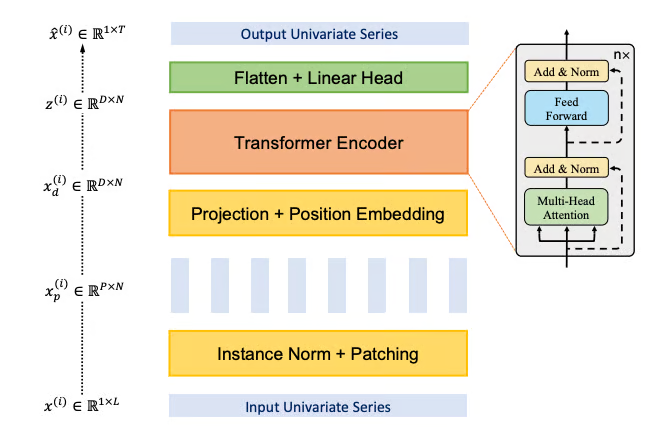
\includegraphics[width=\linewidth,height=54mm,keepaspectratio]{../figures/patchtst.png}
\smallnote{Source: Nie et al., \textit{A Time Series is Worth 64 Words}, ICLR 2023. Same architecture illustration as thesis Chapter 2.}
\column{.36\textwidth}
\small\textbf{Our selected raw model}
\begin{itemize}
\item 30 signal samples; one channel.
\item Patches of 10, stride 2: 11 tokens.
\item Width 128; 4 attention heads; 3 encoder layers.
\item Flatten + linear head: 10 future values at once.
\end{itemize}
\smallnote{The figure shows the original normalization step. Our forecaster has no internal instance normalization: raw or context-standard input is prepared externally.}
\end{columns}
\end{frame}

\begin{frame}[noframenumbering]{B12 | Autoregressive Models: Exact Inputs}
\small $x_t=[S_{t-29},\ldots,S_t]$: one signal channel, sampled every 30 seconds.\par
\vspace{3mm}
\renewcommand{\arraystretch}{1.35}
\begin{tabularx}{\textwidth}{@{}>{\raggedright\arraybackslash}p{59mm}>{\raggedright\arraybackslash}X@{}}
\toprule
Model / task & Input for one prediction\\\midrule
GRU S2V, GRU encoder--decoder, PatchTST & $30\times1$ sequence: $x_t$ or $(x_t-\mu_t)/s_t$. No scalar features.\\
XGBoost / autoregressive & Same 30 raw or standardized lags, flattened. One regressor per future step.\\
Chronos zero-shot & Raw vector of 30 or 120 samples; internal scaling and tokenization.\\
\bottomrule
\end{tabularx}\par
\vspace{3mm}
\textbf{Raw and context-standard are separate runs.}\par
$\mu_t$ and $s_t$ come only from the input window. Standardized forecasts are transformed back with those same statistics.
\smallnote{Shapes exclude the batch dimension. All models output ten future signal values. No scalar summaries, timestamps or meteorological covariates are appended.}
\end{frame}

\begin{frame}[noframenumbering]{B13 | Persistence Models: Exact Inputs}
\small $x_t=[S_{t-29},\ldots,S_t]$,\quad
$r_t=x_t-S_t$,\quad $q_t=x_t-10$.\par
\vspace{3mm}
\renewcommand{\arraystretch}{1.28}
\begin{tabularx}{\textwidth}{@{}>{\raggedright\arraybackslash}p{59mm}>{\raggedright\arraybackslash}X@{}}
\toprule
Model / task & Input for one prediction\\\midrule
Three shapelet models / current-level & $r_t$: $30\times1$ sequence + 12 scalars through a separate embedding.\\
XGBoost / current-level & $[r_t;\,s_t^{\mathrm{CLP}}]$: 42 tabular features.\\
TCN, shapelet convolution / long-fade & $q_t$: $30\times1$ sequence + 14 scalars through a separate embedding.\\
XGBoost / long-fade & $[q_t;\,s_t^{\mathrm{LFD}}]$: 44 tabular features.\\
Selected XGBoost-AFT / survival & 30 raw lags only; no scalar features.\\
Selected TCN / survival & $r_t$: $30\times1$ sequence + 18 scalars through a separate embedding.\\
\bottomrule
\end{tabularx}
\smallnote{Neural models concatenate the scalar embedding with the encoded sequence/shapelets before the output head. Trees concatenate scalar values with lags. Scalar definitions: B14.}
\end{frame}

\begin{frame}[noframenumbering]{B14 | What Is in the Scalar Context?}
\small
\textbf{Ten shared trailing-window summaries}\par\vspace{1mm}
Mean, standard deviation, minimum, maximum and range of the 30 samples;\par
$S_t-S_{t-1}$, $S_t-S_{t-2}$, $S_t-S_{t-4}$; mean and standard deviation of the last five samples.\par
\vspace{3mm}
\renewcommand{\arraystretch}{1.35}
\begin{tabularx}{\textwidth}{@{}>{\raggedright\arraybackslash}p{31mm}>{\raggedright\arraybackslash}X@{}}
\toprule
Task & Added to those ten summaries\\\midrule
Current-level (12) & $S_t$ and $S_t-0.5$: absolute level and level-recovery boundary.\\
Long-fade (14) & $S_t$, $S_t-10$, elapsed event time and observed sample count since onset.\\
Survival TCN (18) & The long-fade feature types, with survival-event onset; plus current threshold status, time since last above-threshold sample, consecutive below-threshold count and above-threshold fraction in the last five event-local samples.\\
\bottomrule
\end{tabularx}
\par\vspace{3mm}
These features restore absolute level and summarize recent changes or event state; they are not extra sensor measurements.
\smallnote{Feature scaling is fitted on training data during selection. No future event end, target duration or censoring label enters the input. Selected AFT does not use this scalar branch.}
\end{frame}


\end{document}
